\documentclass[aspectratio=169]{beamer}

\usepackage[russian]{babel}
\usepackage{amsfonts}
\usepackage{amsmath}
\usepackage{amssymb}
% \usepackage[cp1251]{inputenc}
\usepackage[utf8]{inputenc}
\usepackage{epigraph}
\usepackage{tikz}
\usepackage{xcolor}
\usepackage{verbatimbox}
\usepackage{pgfplots}
\pgfplotsset{width=10cm,height=6cm,compat=1.3}
\usepackage{pgfplots} 
\usepgflibrary{arrows}


\usetheme{Madrid}

\newcommand{\SubItem}[1]{
    {\setlength\itemindent{15pt} \item[-] #1}
}

\newcommand*{\sele}[1]{{\bf #1}}
\newcommand*{\sel}[1]{\textcolor{blue}{#1}}
\newcommand*{\prob}[1]{\textcolor{magenta}{#1}}
\newcommand*{\vs}[0]{\vspace{10pt}}
\newcommand<>{\fullsizegraphic}[1]{
%  \begin{textblock*}{0cm}(-1cm,-3.78cm)
  \includegraphics[width={\paperwidth}]{#1}
%  \end{textblock*}
}

\title[Про Диссернет]{Про Диссернет}
\author{Павел Айткулов}
\institute[]{ajtkulov@gmail.com, Orb Intelligence / Dun and Bradstreet}
\date{28 Sep 2022}

\begin{document}

\frame{\titlepage}

\frame
{
\frametitle{Обо мне}

\begin{itemize}
  \item data-, ML-engineer
  \item scala, fp
  \item спортивное ЧГК, Puzzle, top-250
  \item шахматы, $Elo = 2050 \ldots 2100, Elo_{max} = 2118$
  \item бег, марафон: 3h 57m (2019), $\frac{1}{2}$ марафон: 1h 42m, 10k: 44m 30s (2021)
  \item русский бильярд
\end{itemize}


}



\frame
{
\frametitle{Диссернет}

Диссернет
\href{https://www.dissernet.org/}{https://www.dissernet.org/}


\vspace{3mm}
Что, Где, Когда, Начало 

\vspace{3mm}
\href{https://www.dissernet.org/expertise/andriyanovav2011.htm}{https://www.dissernet.org/expertise/andriyanovav2011.htm}


\vspace{3mm}

Сообщество, но не формальная организация.

\vspace{3mm}

\pause

Атаки/обвинения, не политика. Quis custodiet ipsos custodes?

Ошибки, извинения.

\vspace{1mm}

\href{https://www.dissernet.org/publications/poselyugina_errata.htm}{https://www.dissernet.org/publications/poselyugina\_errata.htm}

}


\frame {
  \frametitle{Количество метаданных и файлов диссертаций}

  \begin{tikzpicture}

  \pgfplotstableread[row sep=\\,col sep=&]{
    interval  & allD  & allEx \\
    1995      & 10234 & 777   \\
    1996      & 10589 & 1100  \\
    1997      & 12269 & 3137  \\
    1998      & 14993 & 10588 \\
    1999      & 17503 & 17125 \\
    2000      & 21282 & 21027 \\
    2001      & 16986 & 16795 \\
    2002      & 23371 & 23166 \\
    2003      & 24454 & 24270 \\
    2004      & 33346 & 33162 \\
    2005      & 33131 & 32926 \\
    2006      & 35250 & 35010 \\
    2007      & 27581 & 27009 \\
    2008      & 23793 & 23304 \\
    2009      & 29845 & 29303 \\
    2010      & 24051 & 23628 \\
    2011      & 26124 & 25502 \\
    2012      & 21321 & 20357 \\
    2013      & 21712 & 20760 \\
    2014      & 13064 & 12548 \\
    2015      & 14843 & 13002 \\
    2016      & 11926 & 10043 \\
    2017      & 11056 & 10252 \\
    2018      & 10880 & 10541 \\
    2019      & 9599  & 9121  \\
    2020      & 7968  & 6168  \\
    }\mydata
 
    \begin{axis}[
            ybar,
            bar width=.06cm,
            scaled y ticks=false,
            x tick label style = {font = \small, text width = 1.7cm, align = center, rotate = 70, anchor = north east},
            symbolic x coords={1995, 1996, 1997, 1998, 1999, 2000, 2001, 2002, 2003, 2004, 2005, 2006, 2007, 2008, 
            2009, 2010, 2011, 2012, 2013, 2014, 2015, 2016, 2017, 2018, 2019, 2020},
            xtick=data,
            width=15cm, height=7cm
        ]
        \addplot table[x=interval,y=allD]{\mydata};
        \addplot table[x=interval,y=allEx]{\mydata};
        \legend{MetaData, File};
    \end{axis} 
\end{tikzpicture}

}


\frame {
  \frametitle{Экономисты против технарей}

  \begin{tikzpicture}

  \pgfplotstableread[row sep=\\,col sep=&]{
    interval  & allE & allT & allM \\
    1995      & 949  & 2215 & 1366 \\
    1996      & 1136 & 2295 & 1281 \\
    1997      & 1336 & 2534 & 1424 \\
    1998      & 1786 & 3170 & 1621 \\
    1999      & 2474 & 3627 & 1526 \\
    2000      & 3419 & 4398 & 1594 \\
    2001      & 2581 & 3301 & 1275 \\
    2002      & 3783 & 4341 & 1500 \\
    2003      & 4178 & 3979 & 1436 \\
    2004      & 5458 & 4942 & 1728 \\
    2005      & 5208 & 4606 & 1589 \\
    2006      & 5922 & 5181 & 1822 \\
    2007      & 4668 & 4282 & 1463 \\
    2008      & 3729 & 3391 & 1422 \\
    2009      & 4599 & 4450 & 1501 \\
    2010      & 3826 & 3813 & 1555 \\
    2011      & 4098 & 4340 & 1596 \\
    2012      & 3685 & 3902 & 1346 \\
    2013      & 2822 & 4407 & 1536 \\
    2014      & 1590 & 2578 & 1154 \\
    2015      & 1630 & 2814 & 1095 \\
    2016      & 936  & 2524 & 1142 \\
    2017      & 735  & 2204 & 921  \\
    2018      & 700  & 2250 & 953  \\
    2019      & 637  & 2006 & 804  \\
    2020      & 544  & 1634 & 637  \\
    }\mydata
 
    \begin{axis}[
            ybar,
            bar width=.06cm,
            scaled y ticks=false,
            x tick label style = {font = \small, text width = 1.7cm, align = center, rotate = 70, anchor = north east},
            symbolic x coords={1995, 1996, 1997, 1998, 1999, 2000, 2001, 2002, 2003, 2004, 2005, 2006, 2007, 2008, 
            2009, 2010, 2011, 2012, 2013, 2014, 2015, 2016, 2017, 2018, 2019, 2020},
            xtick=data,
            width=15cm, height=7cm
        ]
        \addplot table[x=interval,y=allE]{\mydata};
        \addplot table[x=interval,y=allT]{\mydata};
        \addplot table[x=interval,y=allM]{\mydata};
        \legend{Economy, Tech, Physical and mathematical};
    \end{axis} 
\end{tikzpicture}

}

\frame {
  \frametitle{Кандидаты против Докторов}

  \begin{tikzpicture}

  \pgfplotstableread[row sep=\\,col sep=&]{
    interval  & allD & allP \\
    1995      & 1948 & 8282 \\
    1996      & 2019 & 8565 \\
    1997      & 2514 & 9749 \\
    1998      & 2896 & 12088 \\
    1999      & 3077 & 14420 \\
    2000      & 3165 & 18110 \\
    2001      & 2718 & 14259 \\
    2002      & 3036 & 20322 \\
    2003      & 3269 & 21174 \\
    2004      & 4149 & 29183 \\
    2005      & 3915 & 27761 \\
    2006      & 4144 & 31096 \\
    2007      & 2989 & 24580 \\
    2008      & 2426 & 21350 \\
    2009      & 3653 & 26165 \\
    2010      & 2770 & 21273 \\
    2011      & 3260 & 22852 \\
    2012      & 2706 & 18610 \\
    2013      & 2379 & 19329 \\
    2014      & 1600 & 11448 \\
    2015      & 1861 & 12970 \\
    2016      & 1439 & 10485 \\
    2017      & 1374 & 9680 \\
    2018      & 1393 & 9479 \\
    2019      & 1238 & 8339 \\
    2020      & 1034 & 6927 \\
    }\mydata
 
    \begin{axis}[
            ybar,
            bar width=.06cm,
            scaled y ticks=false,
            x tick label style = {font = \small, text width = 1.7cm, align = center, rotate = 70, anchor = north east},
            symbolic x coords={1995, 1996, 1997, 1998, 1999, 2000, 2001, 2002, 2003, 2004, 2005, 2006, 2007, 2008, 
            2009, 2010, 2011, 2012, 2013, 2014, 2015, 2016, 2017, 2018, 2019, 2020},
            xtick=data,
            width=15cm, height=7cm
        ]
        \addplot table[x=interval,y=allD]{\mydata};
        \addplot table[x=interval,y=allP]{\mydata};
        \legend{Dr of Science, Phd};
    \end{axis} 
\end{tikzpicture}

}


\frame {
  \frametitle{Тезаурус}

\begin{itemize}
  \item карбункул, нарезка. \href{https://www.dissernet.org/expertise/danilinalyu2012.htm}{https://www.dissernet.org/expertise/danilinalyu2012.htm}, \href{https://www.dissernet.org/expertise/ramazanovakk2011_.htm}{https://www.dissernet.org/expertise/ramazanovakk2011\_.htm}
  \item ЗОЛУС, новояз (зоДлус)
  \item ВАК, МинОбр, Диссовет
  \item фантом 
  \item иностранцы, <<таджики>>. Без коннотаций национализма или расизма
  \item фабрики, Машина времени, 10 лет для срока давности и после 2010 года

\end{itemize}
}

\frame {
  \frametitle{Плагиат}




\begin{itemize}

\item текстовый
\item численный, табличный
\item иной

\end{itemize}

Копирование текста или чисел, но не идей. \par

Очевидно доказывать, за исключением терВера, <<Война и мир>> с заменой 1 буквы.

\vspace{1mm}
{\color{blue}{
<<Барак Обама 18 сентября посетил Токио с рабочим визитом.>>

\vspace{1mm}

<<Президент США прибудет в столицу Японии в начале следующей недели.>>
}}
\vspace{5mm}
\pause

Зачем злодеи это делают? Списывание, торговля, криминал.
}


\frame {
  \frametitle {Не только диссертации}

Научные статьи, монографии
\begin{itemize}
  \item Множественные публикации
  \item Самоплагиат
  \item K-кругов ада
  \item Перевод с других языков
  \item П(Б)латные соавторы. Продажа места в соавторах.
\end{itemize}

\pause

Даже в отписке на ЗОЛУС. 

\vspace{3mm}

Патенты, судебные решения, судебные экспертизы.

\vspace{3mm}

Диссеропедия журналов и вузов.

\vspace{3mm}

Ретрагирование статьи. Хищнические журналы.
}

\frame {
  \frametitle{Поток}

Структура защиты, научрук, оппоненты, ведущая организация. Статьи в ВАК.

\vspace{3mm}

Кандидатская и докторская (совместные работы с учениками).

\vspace{3mm}

ЗОЛУС, <<родной>> vs. <<не родной>> диссовет.

\vspace{3mm}

Диссовет, ВАК, МинОбр (в редких случаях, на отрицательное решение Диссовета не смотрят).

\vspace{3mm}

VIP, Экспертный совет ВАК/МинОбр.

\vspace{3mm}

Фантомы.
}

\frame { 
  \frametitle{Статистика на сегодня}

  Ректоры/депутаты/остальные. Все слои населения.
\vspace{3mm}
  Структура по остальным специальностям (экономисты, педагоги, юристы, медики, технари) \par
\vspace{3mm}
  11.5К сильное подозрение, 3К экспертиз, 1000+ ЗОЛУСов. \par
\vspace{3mm}
  250 (из 270) ЗОЛУСов пройдено в 2021 году.
}


\frame {
  \frametitle{Коллаборация}

Основной ДатаСет (2M в метаданных, 1М в наличии, 600К диссертаций, 400К авторефератов, 330 Гб текста).
О чистоте.
\vspace{3mm}
Временной Лаг по оцифровке

\vspace{3mm}
\begin{itemize}
\item E-library(мало в публичном доступе, 14М)
\item cyberleninka (2.6M статей, 200Гб текста)
\item Web
\end{itemize}
\vspace{3mm}

Личности: Википедия, Декларатор

\vspace{3mm}

Аналоги: Антиплагиат (ушли в бизнес), Врониплаг (диссертации, Германия).

}

\frame {
  \frametitle{Текст}

  Версия 1. длинные <<предложения>>. Хеширование, 64 бита. 500М, 10\%

\pause

\vspace{3mm}

  Версия 2. n-gram. 500Гб хешей. $n = 6$, размер не зависит от $n$. 20B n-gram.

\vspace{3mm}

  Отсекаем частотные n-gram, <<На правах рукописи, работа выполнена в>> ($freq \le 5$).
}

\frame {
  \frametitle{Текстовый плагиат в выводах}

  Штрафуется серьезнее.

  \href{https://www.facebook.com/andrei.rostovtsev/posts/4305629239498604}{https://www.facebook.com/andrei.rostovtsev/posts/4305629239498604}

  Выводы. Обычно такие главы начинаются с новой страницы. Отсечь библиографию.
}

\frame {
  \frametitle{Числа}

  Табличный плагиат. После OCR есть разбивка на страницы.
\vspace{3mm}

  Оставляем только нетривиальные числа. 3-gram, хеширование.
\vspace{3mm}

  Страница или соседняя страница содержит подстроку <<ТАБЛИЦ>>.
\vspace{3mm}

  \href{http://wiki.dissernet.org/wsave/LiYuPN2007.html}{http://wiki.dissernet.org/wsave/LiYuPN2007.html}
  \href{https://www.dissernet.org/expertise/melnikovaen2011.htm}{https://www.dissernet.org/expertise/melnikovaen2011.htm}

\vspace{3mm}

  Медики.
}


\frame {
  \frametitle{Числа с подлогом}

  Бежим по графу тектового копирования. Попарно сравниваем таблицы с учетом редакционного расстояния. 2-gram, отдельно для таблиц с $\pm$.

\vspace{3mm}

Сейчас найдено порядка 20 случаев.

\pause

\vspace{3mm}

\href{http://wiki.dissernet.org/wsave/BulatovRN2018.html}{http://wiki.dissernet.org/wsave/BulatovRN2018.html}
\footnote{заменяет последние цифры в результатах исследования везде на единицу}
\vspace{1mm}
\href{http://wiki.dissernet.org/wsave/DmitrenkoGD2014.html}{http://wiki.dissernet.org/wsave/DmitrenkoGD2014.html}
\footnote{2-я табл. Величины и ошибки изменяются на 0.1 (большие величины - на 0.2 и 0.3)}
\vspace{1mm}
\href{http://wiki.dissernet.org/wsave/ParamonovYuO2019.html}{http://wiki.dissernet.org/wsave/ParamonovYuO2019.html}
\footnote{Добавление "0.1" к величинам измерений, погрешности оставлены без изменений.}
\href{http://wiki.dissernet.org/wsave/BalikoevaFR2013.html}{http://wiki.dissernet.org/wsave/BalikoevaFR2013.html}
\footnote{Все погрешности увеличены/уменьшены ровно на 0.2. Величины измерений в 1-й и 4-й строке изменены ровно на 0.12. Во 2-й и 5-й строке - на 0.09 В 3-й и 6-й строке - 1.2}
}


\frame {
  \frametitle{Фуфломицины}
  
  Медицинская мафия. 

  \href{https://ru.wikipedia.org/wiki/\%D0\%91\%D0\%B8\%D0\%BD\%D0\%B3\%D1\%81\%D1\%82\%D0\%B8}{https://ru.wikipedia.org/wiki/Бингсти}
}


\begin{frame}[fragile]
  \frametitle{Фуфломицины - 2}
  
  Версия 1. Фиксированный список <<фуфломицинов>>. 

  \begin{verbatim}
____________ [Термин1] ____________ <----> ____________ [Термин2] ____________

  \end{verbatim}

Замена или добавление медицинского термина. <<Щелкает>> текстовым плагиатом в левом и правом контекстах.

\vspace{3mm}

\pause

Есть граф копирований. Рассматриваем только диссертации биологических, медицинских и фармацевтических наук.

\vspace{3mm}

Найдено порядка 100-150 работ.

\end{frame}


\begin{frame}[fragile]
  \frametitle{Фуфломицины - 3}
  
  Версия 2. ML для определения слова-фармакологии.

  Логистическая регрессия. Общий список слов vs. аптечный каталог. (ROC AUC=0.97)


\end{frame}

\frame {
  \frametitle {VIP}

  Wikipedia - 400K имен, известные и популярные, вся история, пересечения по ФИО, 50\% попаданий.

  Декларатор - 300К имен, кто обязан сдавать декларации о доходах, в том числе работник районной налоговой инспекции.

\vspace{3mm}
  Спортсмены, политики, Контр-адмирал, генералы ФСБ, учителя английского, врачи, губернаторы.

\pause

\vspace{3mm}
  \href{https://www.dissernet.org/expertise/kozlovsv2006.htm}{https://www.dissernet.org/expertise/kozlovsv2006.htm}
  \href{https://ru.wikipedia.org/wiki/\%D0\%9A\%D0\%BE\%D0\%BD\%D1\%82\%D1\%80-\%D0\%B0\%D0\%B4\%D0\%BC\%D0\%B8\%D1\%80\%D0\%B0\%D0\%BB}{https://ru.wikipedia.org/wiki/Контр-адмирал}
  \href{https://ru.wikipedia.org/wiki/\%D0\%9A\%D0\%BE\%D0\%B7\%D0\%BB\%D0\%BE\%D0\%B2,\_\%D0\%A1\%D0\%B5\%D1\%80\%D0\%B3\%D0\%B5\%D0\%B9\_\%D0\%92\%D0\%B8\%D0\%BA\%D1\%82\%D0\%BE\%D1\%80\%D0\%BE\%D0\%B2\%D0\%B8\%D1\%87}{https://ru.wikipedia.org/wiki/Козлов,\_Сергей\_Викторович}

\vspace{3mm}

  Прогоны по кандидатам в ГД РФ.  
}

\frame {
  \frametitle {VIP, quiz}

  \begin{itemize}
    \item 1997, 45 лет, кандидатская, экономических

    \item 1998, 38 лет, кандидатская, экономических

    \item 2000, 59 лет, кандидатская, экономических

\pause

    \item все с одного совета

\pause

    \item 2010, 69 лет (тот же самый человек), докторская, экономических

\pause

    \item в 2021 <<научрук>> (формально, связь сложнее) стал долларовым миллиардером (\$1.5 млрд) \href{https://www.svoboda.org/a/31190795.html}{https://www.svoboda.org/a/31190795.html}

\pause
    \item все <<питерские>>

  \end{itemize}

\pause

Правильные ответы: 

\href{
https://ru.wikipedia.org/wiki/Литвиненко,\_Владимир\_Стефанович}{https://ru.wikipedia.org/wiki/Литвиненко,\_Владимир\_Стефанович}

\vspace{3mm}

Плагиата пока не найдено. На таком уровня вряд ли он есть.

\pause
\vspace{3mm}

Либо <<дареному коню>> \ldots примеры и контр-примеры.

}


\frame{
  \frametitle{Разное}

  Обновление источников
  \href{http://wiki.dissernet.org/wsave/NikogdaYuV2013.html}{http://wiki.dissernet.org/wsave/NikogdaYuV2013.html}

\vspace{3mm}

  Игошенизация (<<шоколад>> $\rightarrow$ <<мясо>>)

  \href{https://www.dissernet.org/expertise/igoshinin2004.htm}{https://www.dissernet.org/expertise/igoshinin2004.htm}

  \par
  
  \href{https://ru.wikipedia.org/wiki/\%D0\%98\%D0\%B3\%D0\%BE\%D1\%88\%D0\%B8\%D0\%BD,\_\%D0\%98\%D0\%B3\%D0\%BE\%D1\%80\%D1\%8C\_\%D0\%9D\%D0\%B8\%D0\%BA\%D0\%BE\%D0\%BB\%D0\%B0\%D0\%B5\%D0\%B2\%D0\%B8\%D1\%87}{https://ru.wikipedia.org/wiki/Игошин,\_Игорь\_Николаевич}
}

\frame {
  \frametitle{Cases}

  \begin{tikzpicture}

  \pgfplotstableread[row sep=\\,col sep=&]{
    interval  & allE & allT \\
    1995      & 1    & 1 \\
    1996      & 4    & 5 \\
    1997      & 3    & 4 \\
    1998      & 8    & 10 \\
    1999      & 72   & 86 \\
    2000      & 124  & 155 \\
    2001      & 132  & 155 \\
    2002      & 256  & 315 \\
    2003      & 438  & 499 \\
    2004      & 806  & 864 \\
    2005      & 942  & 1005 \\
    2006      & 1255 & 1350 \\
    2007      & 1033 & 1144 \\
    2008      & 832  & 929 \\
    2009      & 985  & 1101 \\
    2010      & 864  & 991 \\
    2011      & 1436 & 1667 \\
    2012      & 812  & 1325 \\
    2013      & 184  & 388 \\
    2014      & 79   & 142 \\
    2015      & 53   & 102 \\
    2016      & 22   & 47 \\
    2017      & 13   & 31 \\
    2018      & 0    & 20 \\
    2019      & 0    & 16 \\
    2020      & 0    & 4 \\
    }\mydata
 
    \begin{axis}[
            ybar,
            bar width=.06cm,
            scaled y ticks=false,
            x tick label style = {font = \small, text width = 1.7cm, align = center, rotate = 70, anchor = north east},
            symbolic x coords={1995, 1996, 1997, 1998, 1999, 2000, 2001, 2002, 2003, 2004, 2005, 2006, 2007, 2008, 
            2009, 2010, 2011, 2012, 2013, 2014, 2015, 2016, 2017, 2018, 2019, 2020},
            xtick=data,
            width=15cm, height=7cm
        ]
        \addplot table[x=interval,y=allE]{\mydata};
        \addplot table[x=interval,y=allT]{\mydata};
        \legend{Mar 2021, Aug 2022};
    \end{axis} 
\end{tikzpicture}

}


\frame{
  \frametitle{Разное - 2}
  \href{https://www.facebook.com/serguei.parkhomenko/posts/10225243601346536?comment\_id=10225244642012552}{https://www.facebook.com/serguei.parkhomenko/posts/10225243601346536?comment\_id=10225244642012552}

  \href{https://www.facebook.com/andrei.rostovtsev/posts/4347241862004008}{https://www.facebook.com/andrei.rostovtsev/posts/4347241862004008}

  \href{https://www.facebook.com/andrei.rostovtsev/posts/4342907015770826}{https://www.facebook.com/andrei.rostovtsev/posts/4342907015770826}

  \href{https://novayagazeta.ru/articles/2016/11/02/70390-biblioteka-s-privideniyami}{https://novayagazeta.ru/articles/2016/11/02/70390-biblioteka-s-privideniyami}

  \href{https://novayagazeta.ru/articles/2021/04/22/dissertatsii-oborotni-v-biblioteke-s-privideniiami}{https://novayagazeta.ru/articles/2021/04/22/dissertatsii-oborotni-v-biblioteke-s-privideniiami}

}


\frame{
  \frametitle{Разное - 3}

  \href{https://www.dissernet.org/expertise/bogunovss2012\_.htm}{https://www.dissernet.org/expertise/bogunovss2012\_.htm}

  \href{https://www.dissernet.org/expertise/229/rozhnikovskijar2007.htm}{https://www.dissernet.org/expertise/229/rozhnikovskijar2007.htm}

  \href{https://www.facebook.com/andrei.rostovtsev/posts/pfbid029QK8S9cCDtikad9W7GUk2Fux7PULVZmoSZE35duUUXrH32xyY2uWFRU4TPUpyqojl}{https://www.facebook.com/andrei.rostovtsev/posts/pfbid029QK8S9...}

  \href{https://www.dissernet.org/expertise/murahovskyag2013.htm}{https://www.dissernet.org/expertise/murahovskyag2013.htm}
}


\frame{
  \frametitle{Журналы-клоны}

Hijacked journals

\vspace{5mm}

Анна Абалкина: Мошеннические сайты, которые используют название, ISSN и другие метаданные оригинальных журналов для обмана потенциальных авторов.

\href{https://trv-science.ru/2021/06/ostorozhno-zhurnaly-klony/}{https://trv-science.ru/2021/06/ostorozhno-zhurnaly-klony/} 

}


\frame{
  \frametitle{Переводные статьи}

\href{https://www.mv.helsinki.fi/home/kopotev/Kutuzov\_etc\_clustering-comparable-corpora\_2016.pdf}{https://www.mv.helsinki.fi/home/kopotev/Kutuzov\_etc\_clustering-comparable-corpora\_2016.pdf}

\href{https://www.dissernet.org/publications/svoboda\_perevodnoy\_plagiat.htm}{https://www.dissernet.org/publications/svoboda\_perevodnoy\_plagiat.htm}

\href{http://wiki.dissernet.org/wsave/IJICC\_2019\_10\_1publ.html}{http://wiki.dissernet.org/wsave/IJICC\_2019\_10\_1publ.html}

\href{http://rosvuz.dissernet.org/person/111797}{http://rosvuz.dissernet.org/person/111797}

}


\frame {
  \frametitle{Дополнительно}
  \href{https://ru.wikipedia.org/wiki/\%D0\%9A\%D0\%BE\%D0\%BC\%D0\%B8\%D1\%81\%D1\%81\%D0\%B8\%D1\%8F\_\%D0\%BF\%D0\%BE\_\%D0\%B1\%D0\%BE\%D1\%80\%D1\%8C\%D0\%B1\%D0\%B5\_\%D1\%81\_\%D0\%BB\%D0\%B6\%D0\%B5\%D0\%BD\%D0\%B0\%D1\%83\%D0\%BA\%D0\%BE\%D0\%B9}{https://ru.wikipedia.org/wiki/Комиссия\_по\_борьбе\_с\_лженаукой}

  \href{https://ru.wikipedia.org/wiki/\%D0\%9A\%D0\%BE\%D0\%BC\%D0\%B8\%D1\%81\%D1\%81\%D0\%B8\%D1\%8F\_\%D0\%BF\%D0\%BE\_\%D0\%BF\%D1\%80\%D0\%BE\%D1\%82\%D0\%B8\%D0\%B2\%D0\%BE\%D0\%B4\%D0\%B5\%D0\%B9\%D1\%81\%D1\%82\%D0\%B2\%D0\%B8\%D1\%8E\_\%D1\%84\%D0\%B0\%D0\%BB\%D1\%8C\%D1\%81\%D0\%B8\%D1\%84\%D0\%B8\%D0\%BA\%D0\%B0\%D1\%86\%D0\%B8\%D0\%B8\_\%D0\%BD\%D0\%B0\%D1\%83\%D1\%87\%D0\%BD\%D1\%8B\%D1\%85\_\%D0\%B8\%D1\%81\%D1\%81\%D0\%BB\%D0\%B5\%D0\%B4\%D0\%BE\%D0\%B2\%D0\%B0\%D0\%BD\%D0\%B8\%D0\%B9}{https://ru.wikipedia.org/wiki/Комиссия\_по\_противодействию\_\\ фальсификации\_научных\_исследований}

  Увы, у академии мало влияния на государство и процессы. Все в обратную сторону.

\vspace{3mm}

Нет доступа до монографий, статей и диссертаций. Текущий датасет - удача, что в пандемию РГБ ненадолго <<ошибочно выложили>> в открытый доступ. Список МинОбра о существующих защитах не доступен. 

\vspace{3mm}

Научрук после ЗОЛУСа лишается право занимать должность в Диссовете на 5 лет. 

}



\frame{
  \frametitle{Итоги}

\begin{itemize}
  \item Текстовый плагиат (n-gram), диссертации, КиберЛенинка.

  \item Текстовый плагиат, выводы

  \item Табличный плагиат, точное совпадение

  \item Табличный плагиат, подмена

  \item Обновление источников

  \item Фантомы, подозрения на АлтайГУ 2004-2006, аналог СПбГЭУ 2010х.

  \item VIP

  \item Фуфломицины
\end{itemize}

\pause

\vspace{2mm}

  На март 2021 года было 9К (за 2013-2021 годы работы Диссернета) подозрений, на август 2022 - 11.5К. Основные фабрики уже были найдены.

\vspace{2mm}
  2012 год покрыт, 1300+ потенциальных ЗОЛУСОВ. За 2013-2021 подано 1000+ ЗОЛУСов. 
\vspace{2mm}

  Медленно и верно покрываем все, с приоритетом на ЗОЛУСы и срок давности, для 2000-2009 малое покрытие.

}

\frame {
  \frametitle {Links}

  \href{https://www.youtube.com/watch?v=vDKQQSDDj2g}{https://www.youtube.com/watch?v=vDKQQSDDj2g, <<Диссернет. Эволюция альтруизма (научно-популярный фильм)>>}

  \vspace{3mm}

  \href{https://www.youtube.com/c/DissernetTV}{https://www.youtube.com/c/DissernetTV}

  \vspace{3mm}

  \href{https://www.dissernet.org/publications/namedni.htm}{https://www.dissernet.org/publications/namedni.htm} НАМЕДНИ-2013
}

\frame {
  \frametitle{Что дальше?}

  Судебные решения? 

  \href{https://www.dissernet.org/expertise/dudarnn2004.htm}{https://www.dissernet.org/expertise/dudarnn2004.htm}



  \pause 

  Есть датасет. 

\vspace{3mm}

  Другие страны?

\vspace{3mm}

  Идеи?  
}

\frame {
  \frametitle{}

  \begin{figure}
  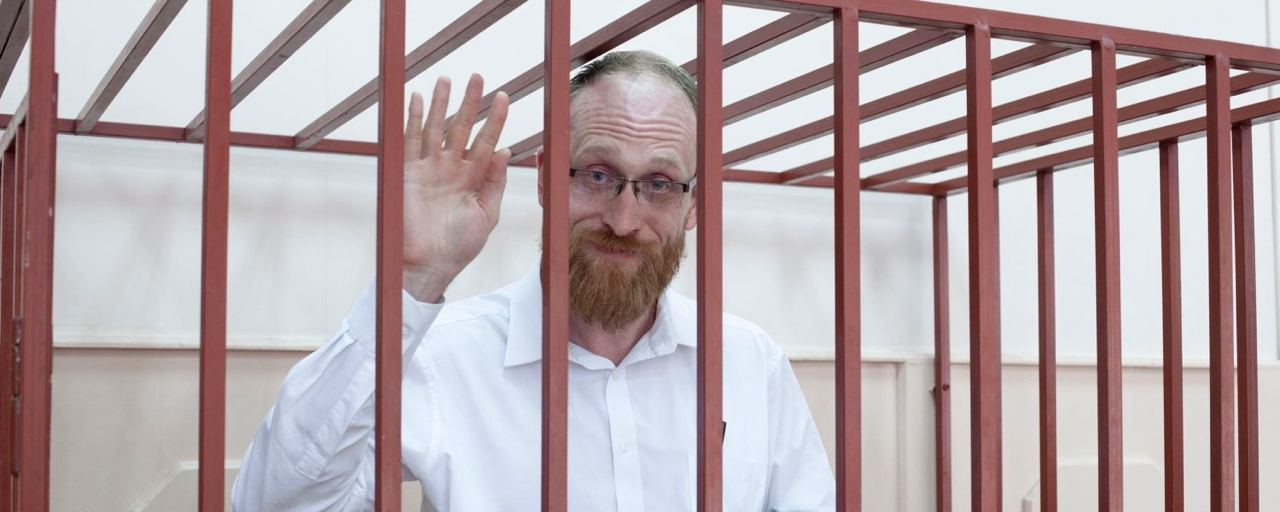
\includegraphics[height=0.4\textwidth]{andrew_z.jpg}
\end{figure}
}

\frame {
  \frametitle{}

  \begin{figure}
  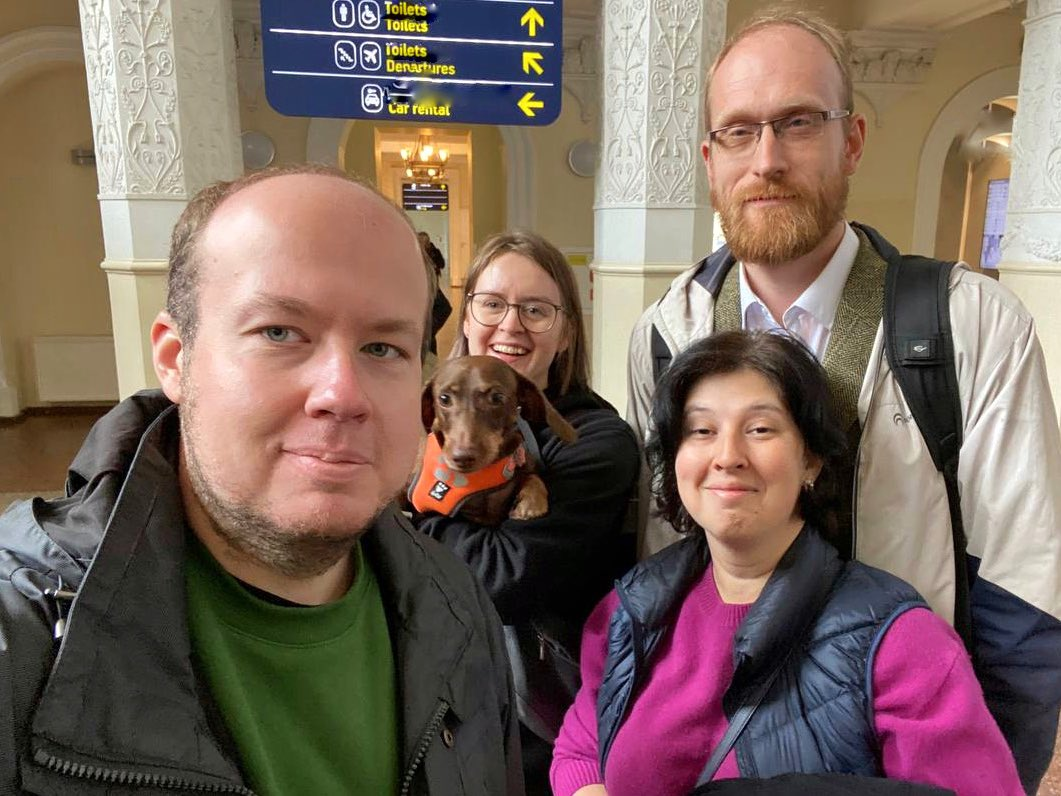
\includegraphics[height=0.6\textwidth]{andrew_after.jpg}
\end{figure}
}













\end{document}